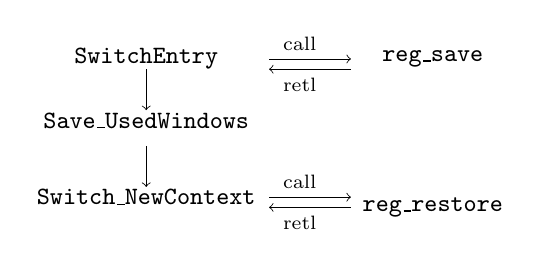
\begin{tikzpicture}[font=\small, line width=0.3pt, scale=1.3]
    \node(SwitchEntry) at (0, 2) {\texttt{SwitchEntry}};
    \node(call0) at (1.5, 2.15) {\scriptsize\text{call}};
    \draw[->] (1.2, 2) -- (2, 2);
    \node(retl0) at (1.5, 1.75) {\scriptsize\text{retl}};
    \draw[->] (2, 1.9) -- (1.2, 1.9);
    \draw[->] (0, 1.9) -- (0, 1.5);
    \node(regsave) at (2.8, 2) {\texttt{reg\_save}};

    \node(SaveUsedWindows) at (0, 1.4) {\texttt{Save\_UsedWindows}};
    \draw[->] (0, 1.15) -- (0, 0.75);

    \node(SwitchNewContext) at (0, 0.65) {\texttt{Switch\_NewContext}};
    \node(call1) at (1.5, 0.8) {\scriptsize\text{call}};
    \draw[->] (1.2, 0.65) -- (2, 0.65);
    \node(retl1) at (1.5, 0.4) {\scriptsize\text{retl}};
    \draw[->] (2, 0.55) -- (1.2, 0.55);
    \node(regrestore) at (2.8, 0.55) {\texttt{reg\_restore}};

    % \node(WindowOK) at (0, 1.4) {\texttt{Window\_OK}};
    % \draw[->] (-0.3, 1.25) -- (-1.6, 0.75);
    % \node(tcneqnull) at (-1.3, 1.2) {\tiny$t_c \neq \text{null}$};
    % \draw[->] (0.3, 1.25) -- (1.8, 0.5);
    % \node(tceqnull) at (1.3, 1.1) {\tiny$t_c = \text{null}$};

    % \node(regsave) at (-2, 0.6) {\texttt{reg\_save}};
    % \draw[->] (-2, 0.5) -- (-2, 0.1);
    % \node(SaveUsedWindows) at (-2, 0) {\texttt{Save\_UsedWindows}};
    % \draw[->] (-1.8, -0.15) -- (-0.5, -0.8);

    % \node(AdjustCWP) at (2, 0.3) {\texttt{Adjust\_CWP}};
    % \draw[->] (2, 0.2) -- (0.4, -0.8);
    % \node(SwitchNewContext) at (0, -0.9) {\texttt{Switch\_NewContext}};

    % \node(regrestore) at (2.8, -0.9) {\texttt{reg\_restore}};
    % \node(call) at (1.5, -0.7) {\tiny\text{call}};
    % \draw[->] (1.2, -0.85) -- (2, -0.85);
    % \node(retl) at (1.5, -1.1) {\tiny\text{retl}};
    % \draw[->] (2, -0.95) -- (1.2, -0.95);
\end{tikzpicture}